\documentclass[border=6pt]{standalone}
\usepackage{fontspec,xeCJK,amsmath,amssymb,tikz,graphicx}
\usetikzlibrary{arrows.meta}
\setmainfont{Arial}\setCJKmainfont{PingFang SC}
\definecolor{ink}{HTML}{203340}\definecolor{blue}{HTML}{147E91}\definecolor{pale}{HTML}{EFF6F5}\definecolor{line}{HTML}{D3E0DF}\definecolor{warm}{HTML}{BA652C}
\begin{document}\begin{tikzpicture}[x=1cm,y=1cm,every node/.style={text=ink,font=\fontsize{10}{13}\selectfont},flow/.style={-{Stealth[length=5pt]},draw=blue,line width=1pt}]
\path[use as bounding box](0,0)rectangle(11,29.2);\fill[pale](0,0)rectangle(11,29.2);
\node[font=\fontsize{19}{23}\selectfont\bfseries]at(5.5,28.4){Transformer：信息不用排队传};
\node[text=blue]at(5.5,27.7){2017 encoder--decoder · base 配置};
\draw[rounded corners=6pt,draw=line,fill=white](.35,22.2)rectangle(10.65,27.0);
\node[anchor=west,font=\fontsize{13}{16}\selectfont\bfseries]at(.65,26.45){A　输入与位置};
\node at(2.15,24.3){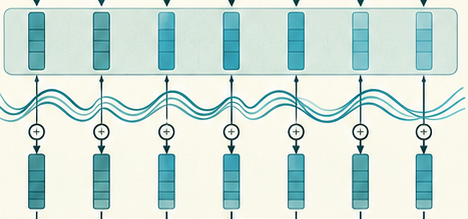
\includegraphics[width=2.8cm,height=2.7cm,keepaspectratio]{visual-1.png}};
\node[anchor=west]at(3.8,25.5){源 token $n\times512$；目标 token $m\times512$};
\node[anchor=west]at(3.8,24.78){嵌入乘 $\sqrt{512}$，加正弦/余弦位置};
\node[anchor=west]at(3.8,24.06){源句进入 B；右移目标前缀进入 C};
\node[anchor=west]at(3.8,23.34){对应正文 §3.4--3.5};
\draw[flow,dotted](5.5,22.2)--(5.5,21.8);
\draw[rounded corners=6pt,draw=line,fill=white](.35,17.0)rectangle(10.65,21.8);
\node[anchor=west,font=\fontsize{13}{16}\selectfont\bfseries]at(.65,21.25){B　编码器：6 层};
\node at(2.15,19.1){
\includegraphics[width=2.8cm,height=2.7cm,keepaspectratio]{visual-2.png}};
\node[anchor=west]at(3.8,20.3){自注意力：Q/K/V 都由本层输入产生};
\node[anchor=west]at(3.8,19.580000000000002){8头 $\times$ 64维 $\to$ 拼接512维};
\node[anchor=west]at(3.8,18.86){前馈 $512\to2048\to512$};
\node[anchor=west]at(3.8,18.14){每个子层：残差相加后 LayerNorm};
\draw[flow,dotted](5.5,17.0)--(5.5,16.6);
\draw[rounded corners=6pt,draw=line,fill=white](.35,11.8)rectangle(10.65,16.6);
\node[anchor=west,font=\fontsize{13}{16}\selectfont\bfseries]at(.65,16.05){C　解码器：6 层};
\node at(2.15,13.900000000000002){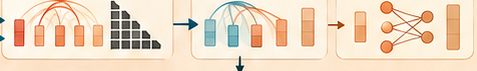
\includegraphics[width=2.8cm,height=2.7cm,keepaspectratio]{visual-3.png}};
\node[anchor=west]at(3.8,15.100000000000001){掩码自注意力：只读前缀};
\node[anchor=west]at(3.8,14.38){交叉注意力：Q来自C，K/V来自B};
\node[anchor=west]at(3.8,13.660000000000002){前馈 $\to$ 词表线性层 $\to$ softmax};
\node[anchor=west]at(3.8,12.940000000000001){下一 token 分布；正文 §3.1--3.3};
\draw[flow,dotted](5.5,11.8)--(5.5,11.4);
\draw[rounded corners=6pt,draw=line,fill=white](.35,6.599999999999999)rectangle(10.65,11.399999999999999);
\node[anchor=west,font=\fontsize{13}{16}\selectfont\bfseries]at(.65,10.849999999999998){D　训练};
\node at(2.15,8.7){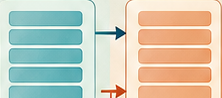
\includegraphics[width=2.8cm,height=2.7cm,keepaspectratio]{visual-4.png}};
\node[anchor=west]at(3.8,9.899999999999999){真值目标右移；因果掩码挡住未来};
\node[anchor=west]at(3.8,9.179999999999998){所有位置并行计算标签平滑交叉熵};
\node[anchor=west]at(3.8,8.459999999999999){梯度更新嵌入、B、C与输出层};
\node[anchor=west]at(3.8,7.739999999999998){Adam；4000步 warm-up；正文 §5};
\draw[flow,dotted](5.5,6.599999999999999)--(5.5,6.199999999999998);
\draw[rounded corners=6pt,draw=line,fill=white](.35,1.3999999999999995)rectangle(10.65,6.199999999999999);
\node[anchor=west,font=\fontsize{13}{16}\selectfont\bfseries]at(.65,5.6499999999999995){E　生成与评估};
\node at(2.15,3.499999999999999){
\includegraphics[width=2.8cm,height=2.7cm,keepaspectratio]{visual-5.png}};
\node[anchor=west]at(3.8,4.699999999999999){源句只编码一次；从起始 token 开始};
\node[anchor=west]at(3.8,3.9799999999999995){生成一个 token，接回C再预测下一个};
\node[anchor=west]at(3.8,3.2599999999999993){BLEU/成本 + 开发集消融；正文 §6};
\node[anchor=west]at(3.8,2.539999999999999){训练并行，不等于生成一步出完整句};
\end{tikzpicture}\end{document}